\graphicspath{{chapters/deep_learning/}}


\chapter{Deep CCA and CCA for Self-Supervised Learning}\label{chap:deep_learning}
\minitoc
% chktex-file 44
% chktex-file 3
\section*{Preface}

\section{Introduction}

\section{Background}

\subsection{DCCA and Deep Multiview CCA}

The goal of DCCA and DMCCA can be defined using our $\MCCA$ notation as maximizing
\begin{align}
    \label{eq:DMCCA-def}
    \norm{\MCCA_K\left(Z\sps{1}, ... Z\sps{I}\right)}_2
\end{align}
over parameters $\theta$ of neural networks defining the representations $Z\sps{i}=f\sps{i}(X\sps{i};\theta\sps{i})$ for $i\in[I]$.

\begin{figure}
    \centering
    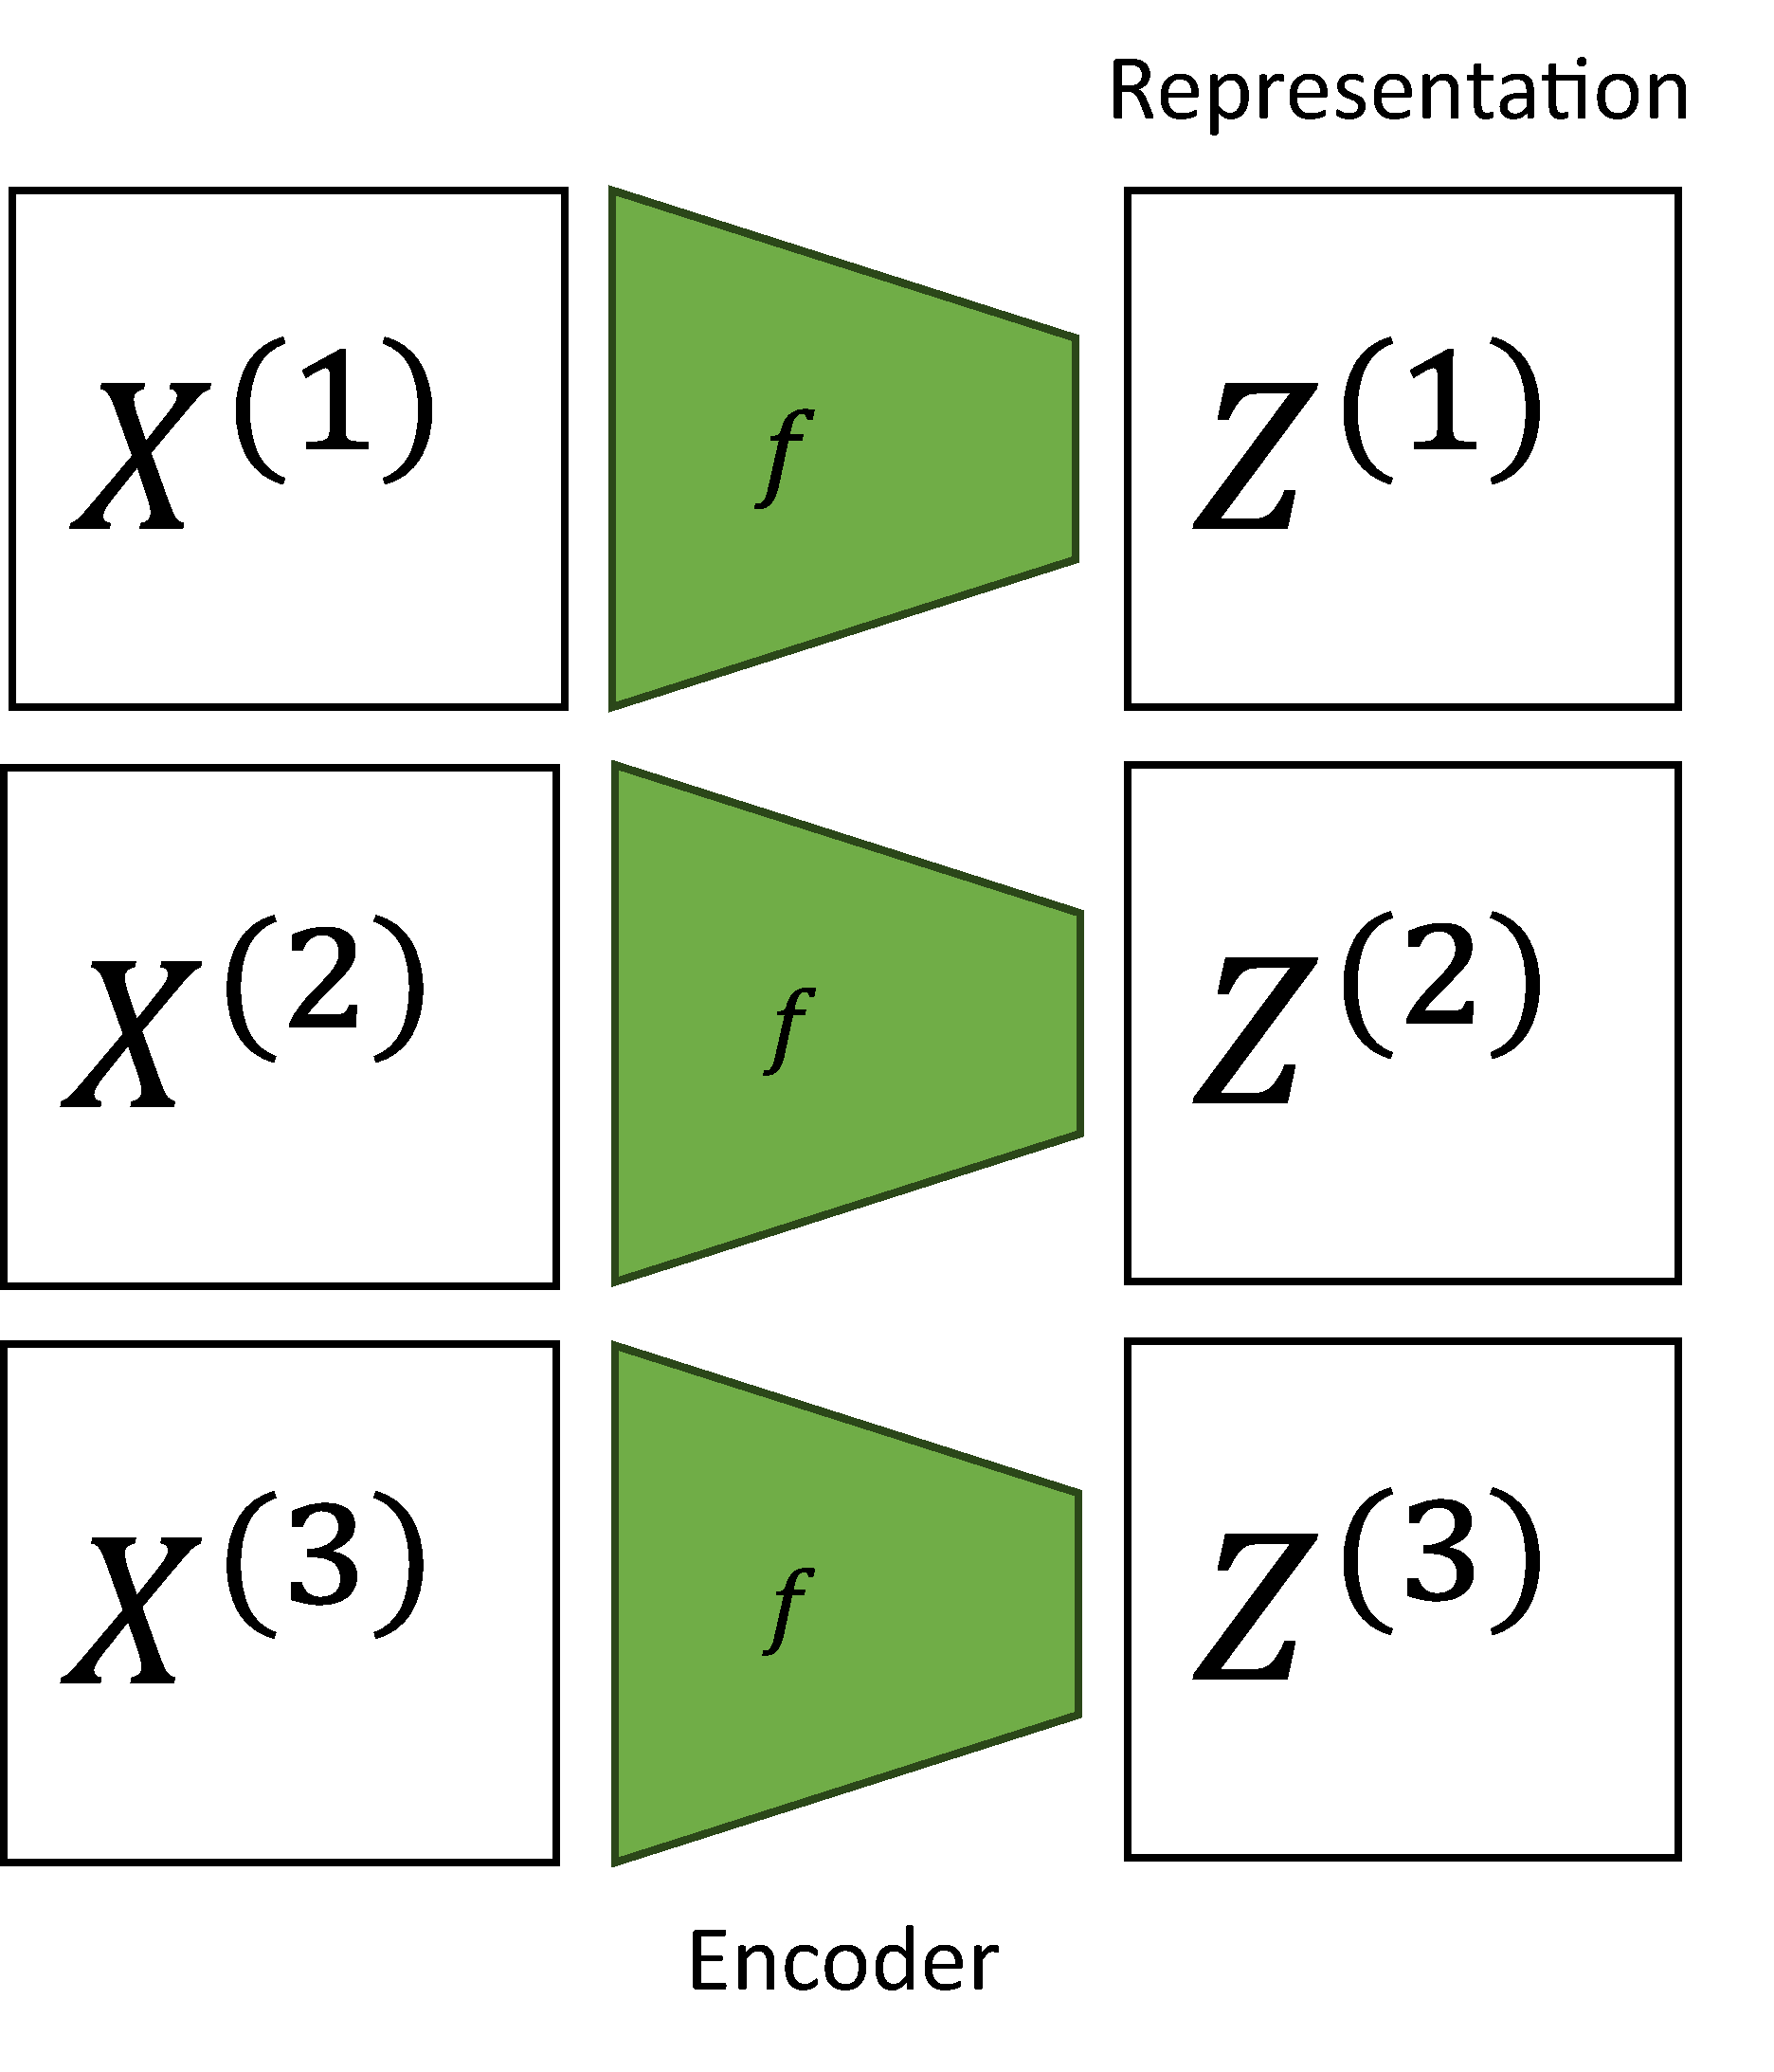
\includegraphics[width=0.4\textwidth]{figures/dcca_schematic}
\end{figure}

The deep canonical correlation analysis (DCCA) landscape comprises three principal approaches with inherent limitations. The first, known as the full-batch approach, uses analytic gradient derivations based on the full sample covariance matrix \citep{andrew2013deep}.
The second involves applying the full batch objective to large mini-batches, an approach referred to as \textbf{DCCA-STOL} \citep{wang2015unsupervised}. However, this approach gives biased gradients and therefore requires batch sizes much larger than the representation size in practice. This is the approach taken by both \textbf{DMCCA} \citep{somandepalli2019multimodal} and \textbf{DGCCA} \citep{benton2017deep} . The final set of approaches use an adaptive whitening matrix \citep{wang2015stochastic, chang2018scalable} to mitigate the bias of the Deep CCA objective. However, the authors of \textbf{DCCA-NOI} highlight that the associated time constant complicates analysis and requires extensive tuning. These limitations make existing DCCA methods less practical and resource-efficient.

\subsection{Self-Supervised Learning}

\begin{figure}
    \centering
    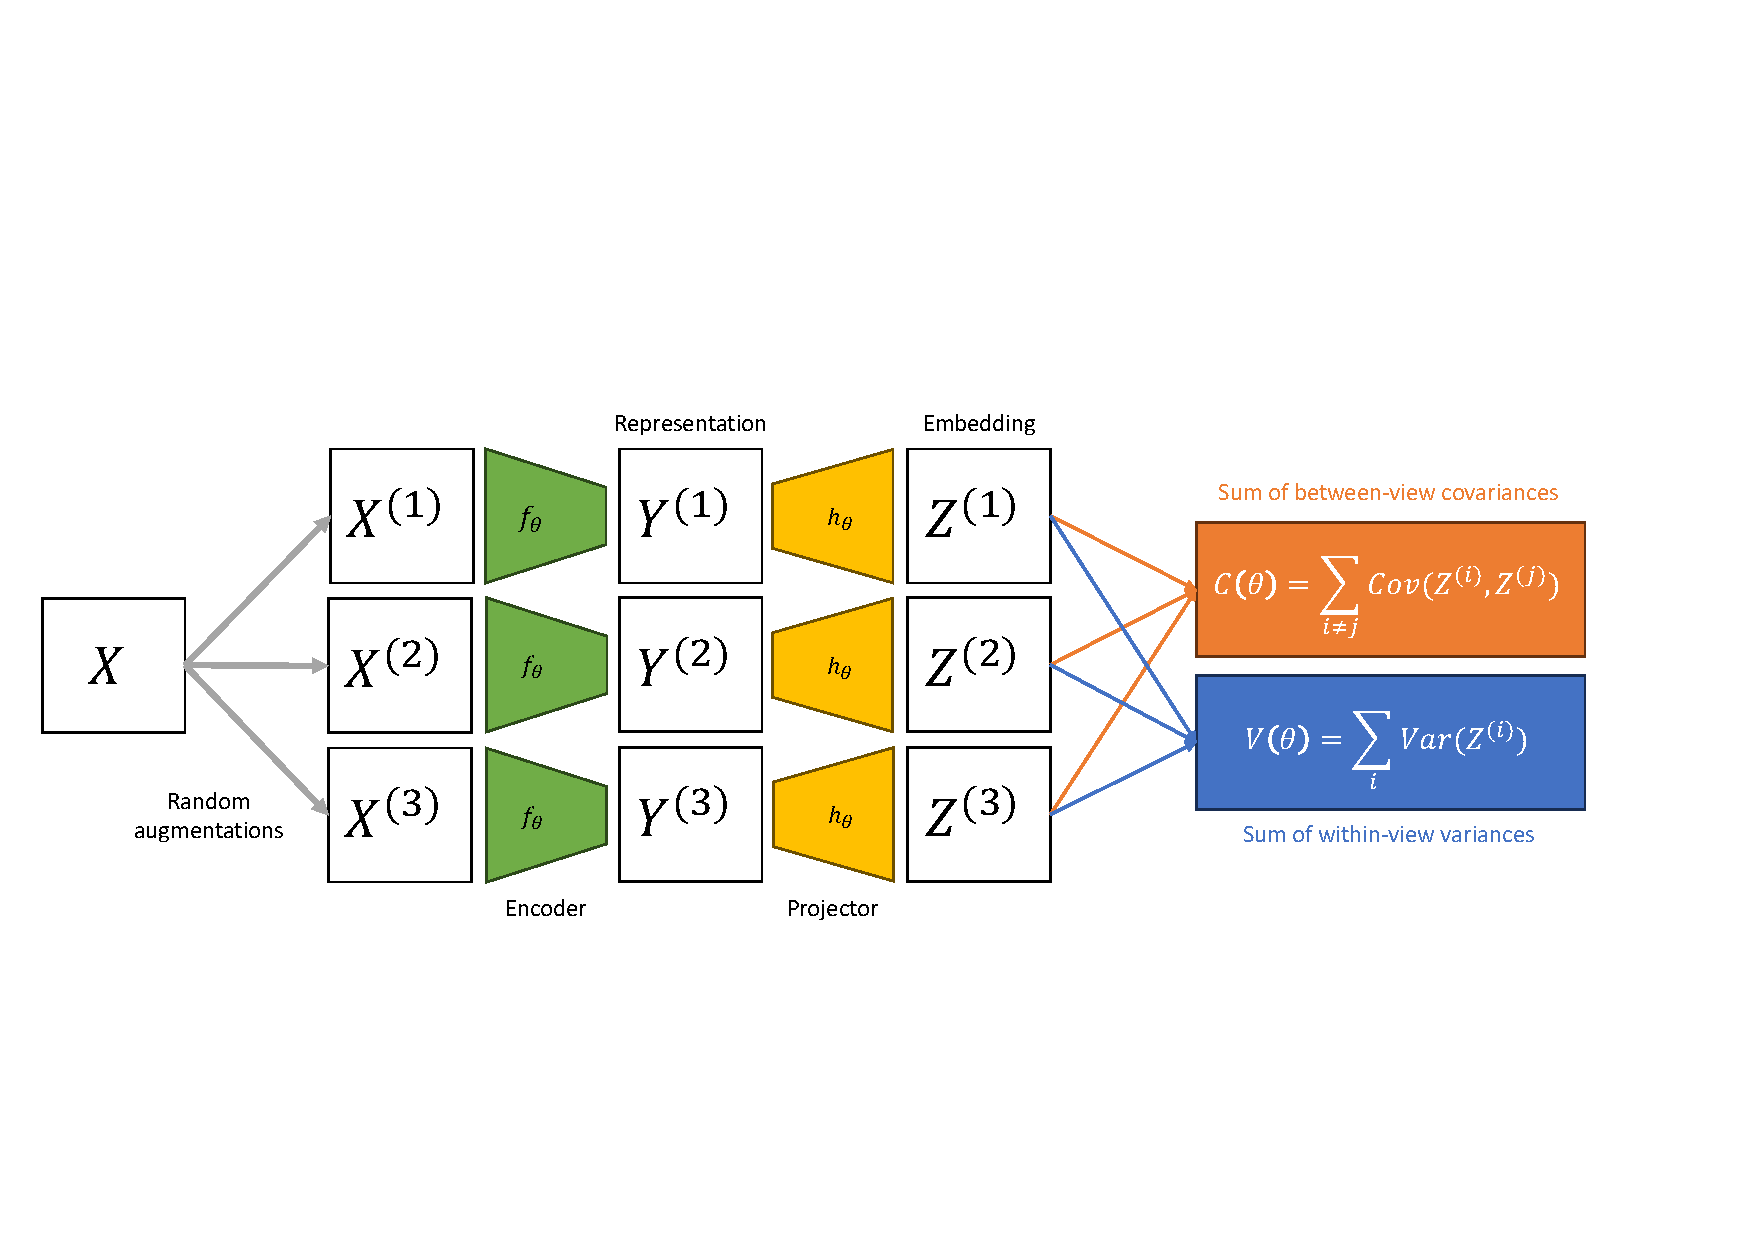
\includegraphics[width=0.8\textwidth]{figures/ssl_schematic}
\end{figure}

\textbf{Barlow Twins} and \textbf{VICReg} have come to be known as part of the canonical correlation family of algorithms \citep{balestriero2023cookbook}. Barlow Twins employs a redundancy reduction objective to make the representations of two augmented views both similar and decorrelated \citep{zbontar2021barlow}. Similarly, VICReg uses variance-invariance-covariance regularization, which draws upon canonical correlation principles, to achieve robust performance in diverse tasks \citep{bardes2021vicreg}. These methods serve as vital baselines for our experiments, owing to their foundational use of canonical correlation ideas.

\section{Methods: Novel Objectives and Algorithms}\label{sec:contributions}

\subsection{Applications to (multi-view) stochastic CCA and PLS, and Deep CCA}
\begin{lemma}[Objective recovers GEP formulation of linear (multi-view) CCA]
    When the $f\sps{i}$ are linear, as in \cref{eq:cca-linear-function-def}, the population loss from \cref{eq:EY-loss-def-C-V} recovers MCCA as defined in \cref{sec:CCA-family}. %Moreover, the minimal loss value is precisely $-\norm{\MCCA_K(X)}$
\end{lemma}
\begin{proof}
    By construction, for linear MCCA we have $C = U^T A U,\, V_\alpha=U^T B_\alpha U$, where $(A, B_\alpha)$ define the GEP for MCCA introduced in \cref{eq:gep-most-general-formulation}.
    So $\LEY(U) = \LEYGEP(U)$ and by \cref{prop:EY-charac} the optimal set of weights define a top-$K$ subspace of the GEP, and so is a MCCA solution.
        %; by definition, $\MCCA_K$ is the vector of top-$K$ generalised eigenvalues, so the optimal value is as claimed.
\end{proof}

Moreover, by following through the chain of back-propagation, we obtain gradient estimates in $\mathcal{O}(MKD)$ time.
Indeed, we can obtain gradients for the transformed variables in $\mathcal{O}(M K^2)$ time so the dominant cost is then updating $U$; we flesh this out with full details in \cref{supp:fast-updates}.

\begin{restatable}{lemma}{recoverDeepCCA}[Objective recovers Deep Multi-view CCA]\label{lem:recover-DeepCCA}
Assume that there is a final linear layer in each neural network $f\sps{i}$.
Then at any local optimum, $\hat{\theta}$, of the population problem, we have
\begin{align*}
    \LEY(\hat{\theta}) = - \norm{\MCCA_K(\hat{Z})}_2^2
\end{align*}
where $\hat{Z} = f_{\hat{\theta}}(X)$.
Therefore, $\hat{\theta}$ is also a local optimum of objectives from \cite{andrew2013deep, somandepalli2019multimodal} as defined in \cref{eq:DMCCA-def}.
\end{restatable}
\begin{proof}[Proof sketch: see \cref{supp:EY-recover-Deep-CCA} for full details.]
    Consider treating the penultimate-layer representations as fixed, and optimising over the weights in the final layer. This is precisely equivalent to optimising the Eckhart-Young loss for linear CCA where the input variables are the penultimate-layer representations. So by \cref{prop:no-spurious}, a local optimum is also a global optimum, and by \cref{prop:EY-charac} the optimal value is the negative sum of squared generalised eigenvalues.
\end{proof}

\subsection{Application to SSL}
We can directly apply Algorithm \ref{alg:general} to SSL.
If we wish to have the same neural network transforming each view, we can simply tie the weights $\theta\sps{1} = \theta\sps{2}$.
When the paired data are generated from applying independent, identically distributed (i.i.d.) augmentations to the same original datum, it is intuitive that tying the weights is a sensible procedure, and perhaps acts as a regulariser.
We make certain notions of this intuition precise for CCA and Deep CCA in \cref{supp:further-cca}.

To provide context for this proposal, we also explored in detail how VICReg and Barlow twins are related to CCA.
For now we focus on VICReg, whose loss can be written as
\begin{small}\begin{align*}
                 \mathcal{L}_\text{VR}(Z\sps{1}, Z\sps{2})
                 &= \gamma \mathbb{E} \norm{Z^{(1)} - Z^{(2)}}^2 + \sum_{i \in \{1,2\}} \bigg[\alpha \sum_{k=1}^K \left(1 \shortminus \sqrt{\Var(Z\sps{i}_i)}\right)_+ + \beta \sum_{\substack{k,l=1 \\ k \neq l}}^K \Cov(Z\sps{i}_k,Z\sps{i}_l)^2 \bigg]
\end{align*}\end{small}%
where $\alpha, \beta, \gamma > 0$ are tuning parameters and, as in the framework of \cref{sec:background-unified}, the $Z\sps{1}, Z\sps{2}$ are $K$-dimensional representations, parameterised by neural networks in \cref{eq:general-form-of-representations}.
Our main conclusions regarding optima of the population loss are:
\begin{itemize}
    \item Consider the linear setting with untied weights. Then global optimisers of the VICReg loss define CCA subspaces, but may not be of full rank.
    \item Consider the linear setting with tied weights and additionally assume that the data are generated by i.i.d. augmentations. Then the same conclusion holds.
    \item In either of these settings, the optimal VICReg loss is a component-wise decreasing function of $\CCA_K(X\sps{1}, X\sps{2})$ the vector of population canonical correlations.
    \item VICReg can therefore be interpreted as a formulation of Deep CCA, but one that will not in general recover full rank representations.
\end{itemize}

% We believe versions of each of these conclusions also hold for Barlow twins, but can only prove a subset of the results at present.%, see \cref{supp:ssl-theory} for further discussion.
We give full mathematical details and further discussion in \cref{supp:ssl-theory}.
The analysis for Barlow twins is more difficult, but we present a combination of mathematical and empirical arguments which suggest all the same conclusions hold, again see \cref{supp:ssl-theory}.

\section{Experiments}\label{Experiments}

% Deep CCA Section

\subsection{Deep CCA}\label{sec:experiments-DCCA}
Second, we compare DCCA-EY against the DCCA methods described in \cref{sec:related-work}. The experimental setup is identical to that of \cite{wang2015stochastic}.
We learn $K=50$ dimensional representations, using mini-batch sizes ranging from 20 to 100 and train for 50 epochs.
Because there is no longer a ground truth we have to use Total Correlation Captured (TCC), given by \( \text{TCC} = \sum_{i=k}^K \rho_k \) where $\rho_k$ are now the empirical correlations between the representations on a validation set.

\textbf{Further details:} As in \citet{wang2015stochastic}, we used multilayer perceptrons with two hidden layers with size 800 and an output layer of 50 with ReLU activations. We train for 20 epochs.

\textbf{Parameters:} For each method, we searched over a hyperparameter grid using \citet{wandb}.

\begin{table}[h!]
    \centering
    \begin{tabular}{|l|l|}
        \hline Parameter           & Values           \\
        \hline minibatch size      & 100, 50, 20      \\
        \hline lr                  & 1e-3, 1e-4, 1e-5 \\
        \hline $\rho$\footnotemark & 0.6, 0.8, 0.9    \\
        \hline epochs              & 50               \\
        \hline
    \end{tabular}
    \footnotetext{$\rho$ is only used for DCCA-NOI}
\end{table}

\textbf{Observations:}
Figure \ref{fig: mnist} compares the methods on the splitMNIST dataset.
DCCA-STOL captures significantly less correlation than the other methods, and breaks down when the mini-batch size is less than the dimension $K=50$ due to low rank empirical covariances.
DCCA-NOI performs similarly to DCCA-EY but requires careful tuning of an additional hyperparameter, and shows significantly slower speed to convergence (Figure \ref{fig:lr_mnist}).

Figure \ref{fig: xrmb} compares the methods on the XRMB dataset.
DCCA-STOL captures significantly less correlation than the other methods, and breaks down when the mini-batch size is less than the dimension $K=50$ due to low rank empirical covariances.
DCCA-NOI performs similarly to DCCA-EY but requires careful tuning of an additional hyperparameter, and shows significantly slower speed to convergence (Figure \ref{fig:lr_mnist}).

\begin{figure}
    \centering
    \begin{subfigure}[b]{0.49\textwidth}
        \centering
        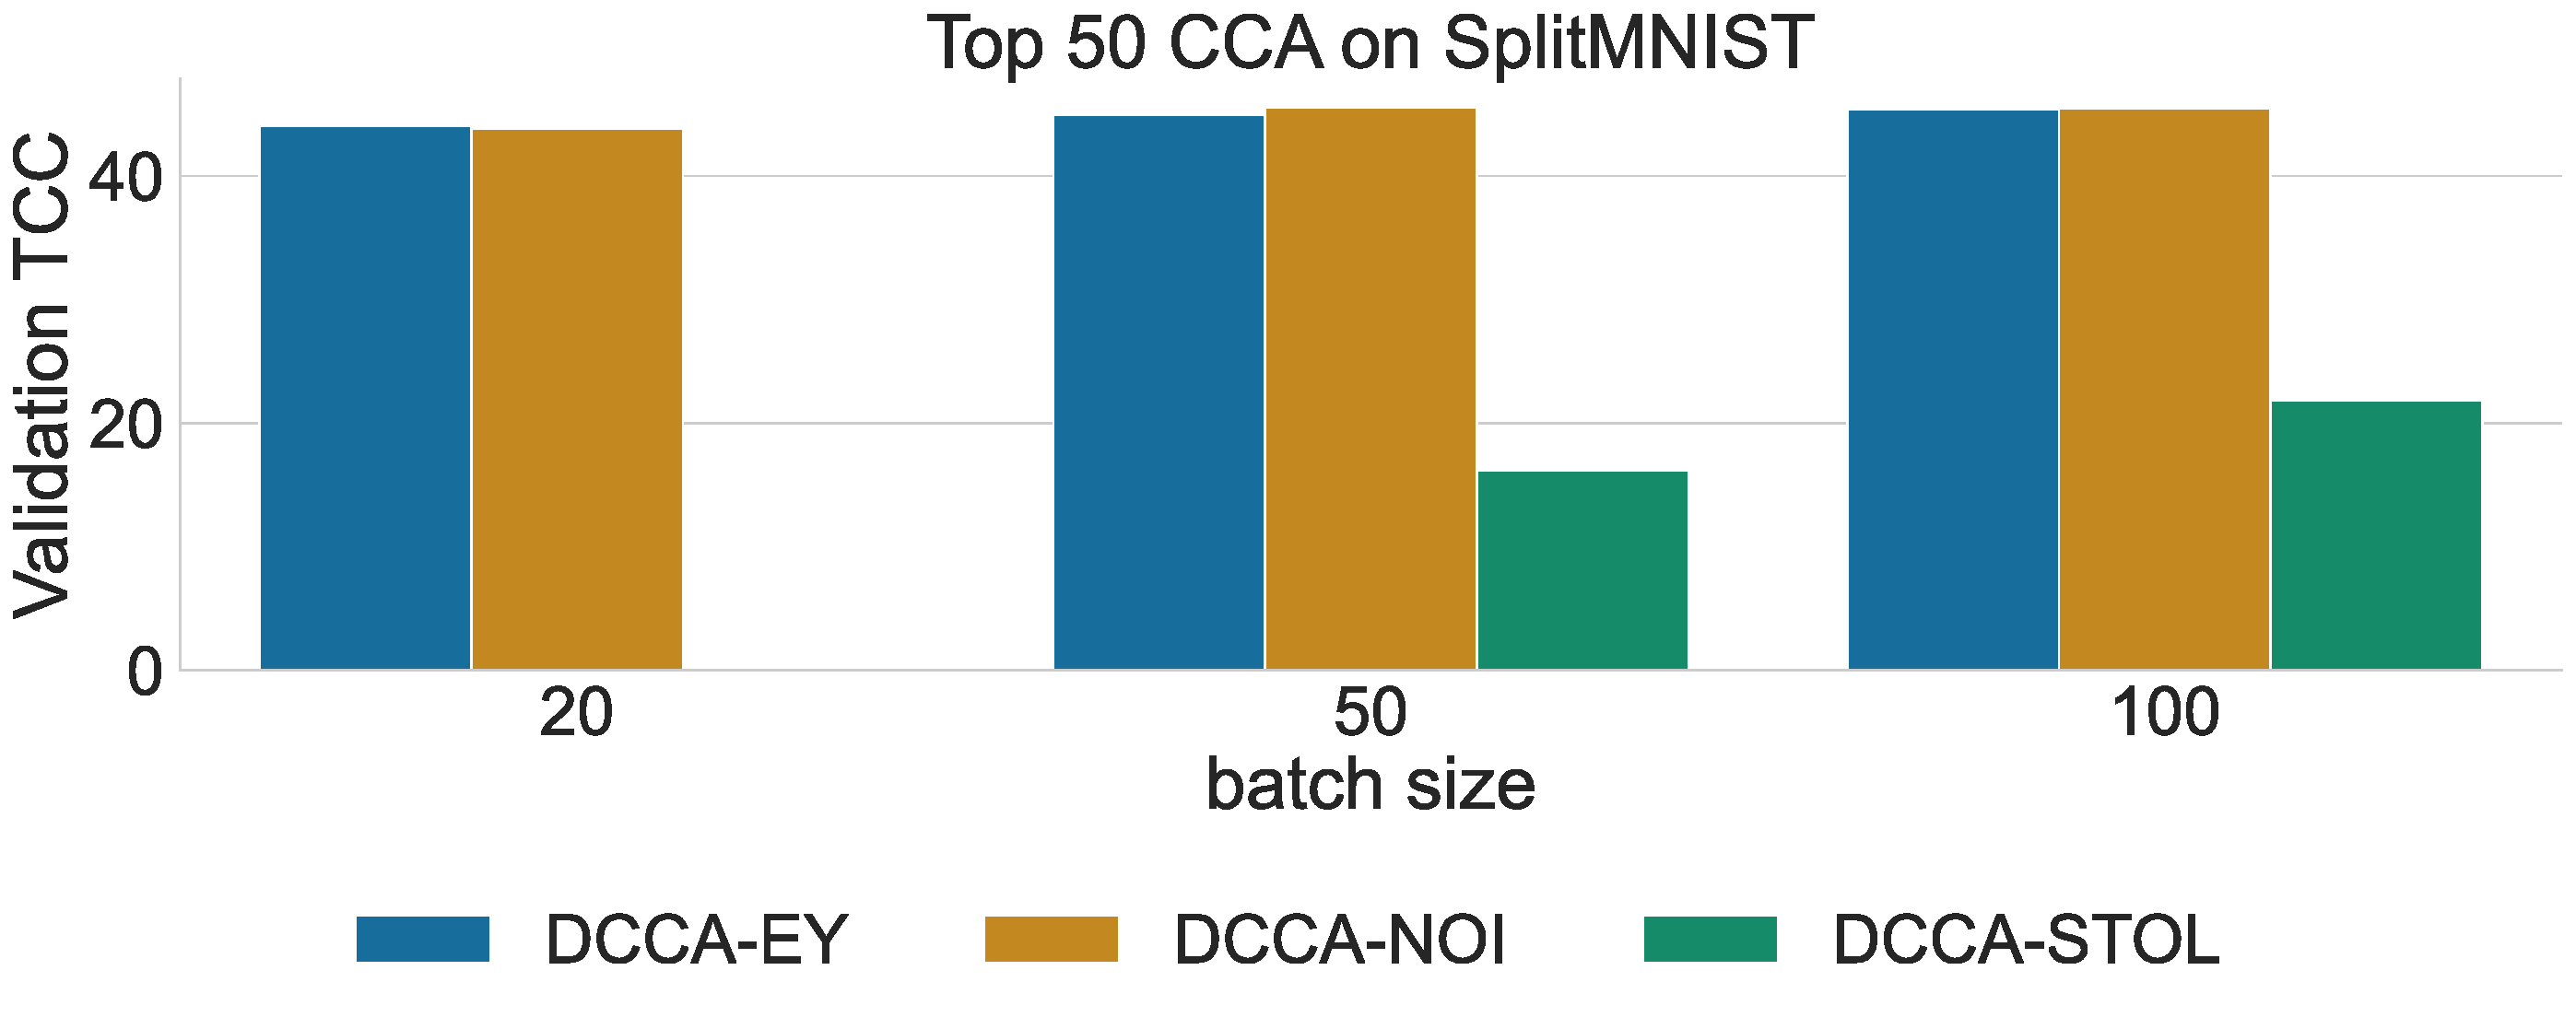
\includegraphics[width=\textwidth]{figures/DCCA/SplitMNIST_models_different_batch_sizes}
        \caption{}
        \label{fig:corr_mnist}
    \end{subfigure}
    \hfill
    \begin{subfigure}[b]{0.49\textwidth}
        \centering
        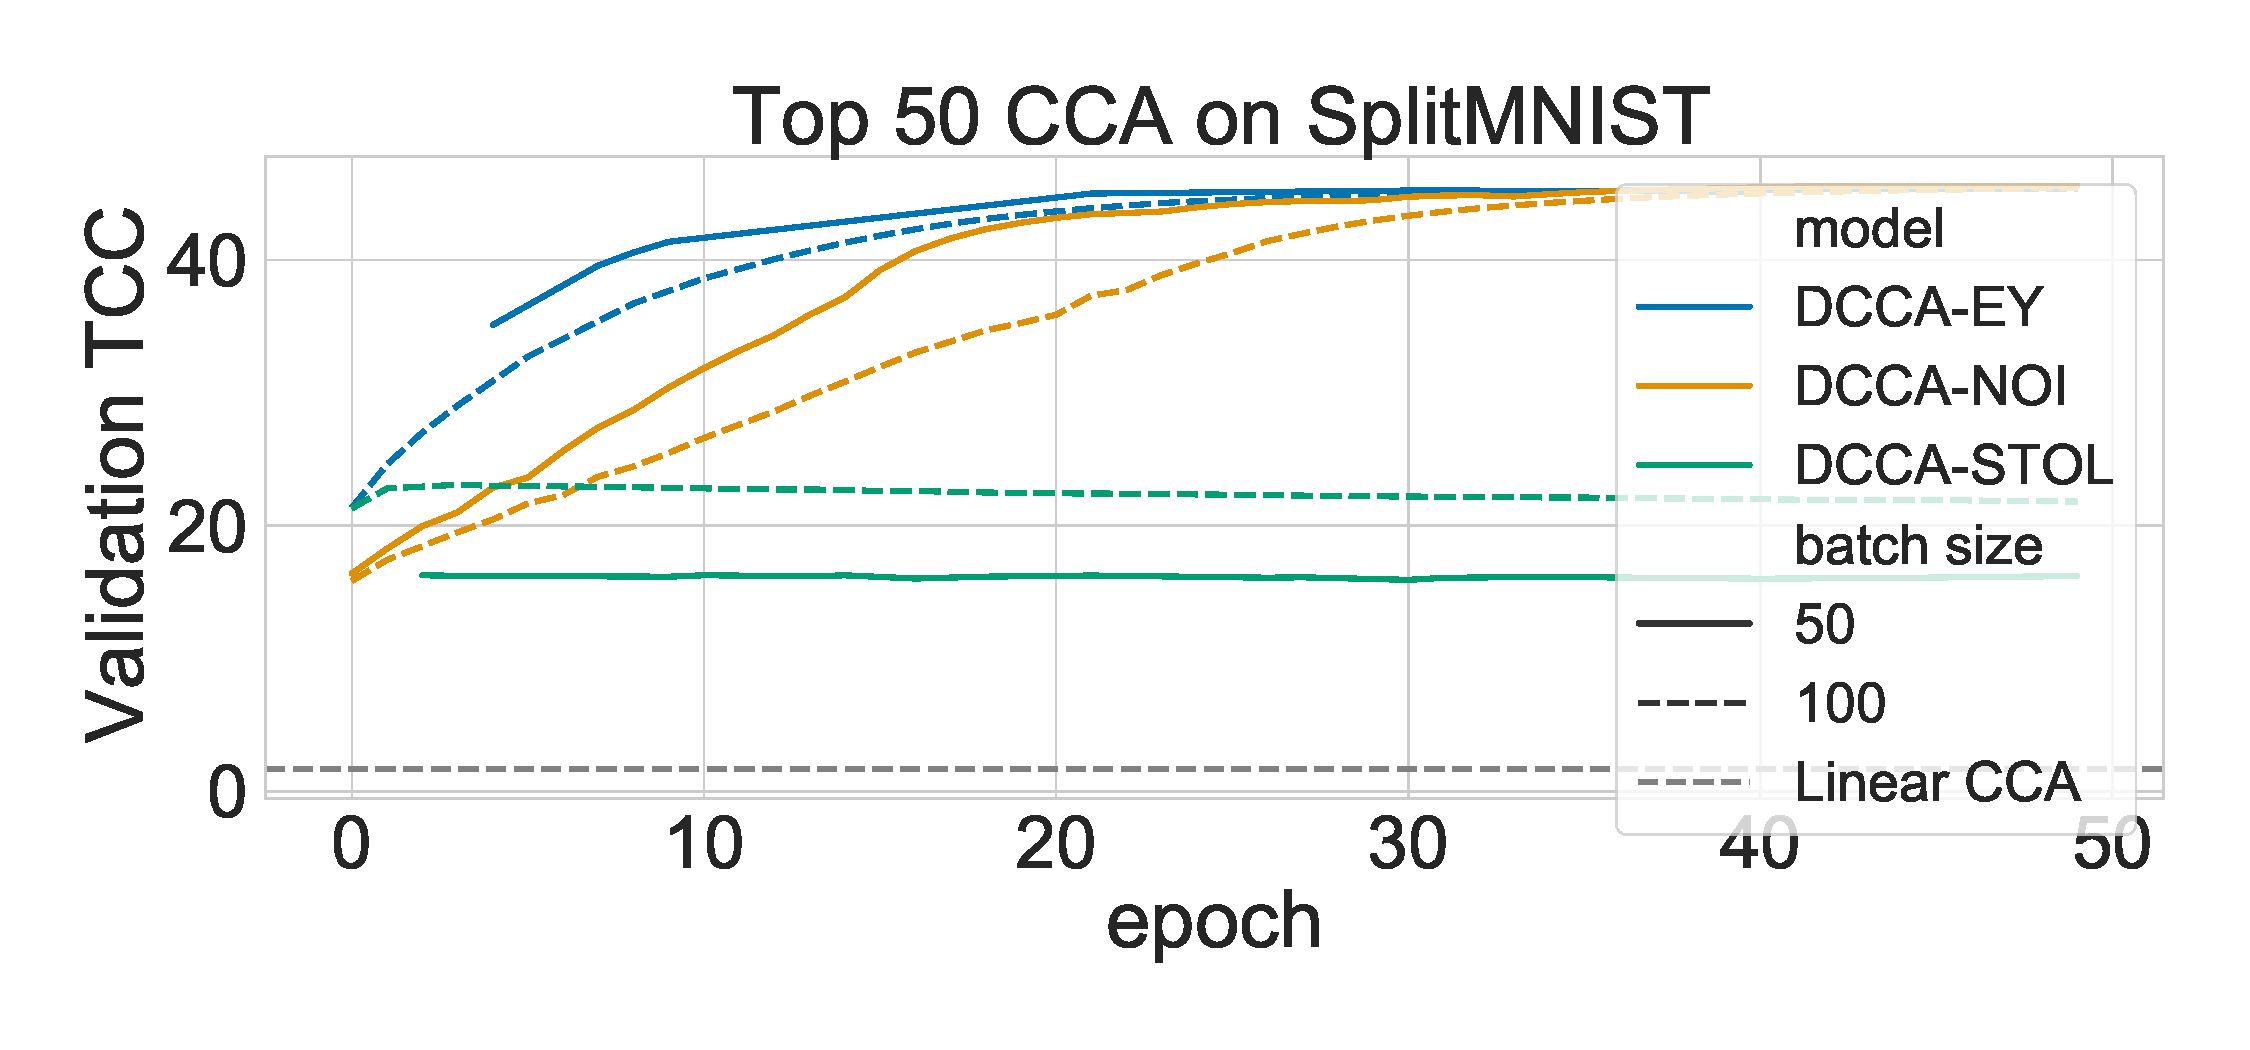
\includegraphics[width=\textwidth]{figures/DCCA/SplitMNIST_allbatchsizes_pcc}
        \caption{}
        \label{fig:lr_mnist}
    \end{subfigure}
    \caption{Deep CCA on SplitMNIST using the Validation TCC metric: (a) after training each model for 50 epochs with varying batch sizes; (b) learning progress over 50 epochs.}
    \label{fig: mnist}
\end{figure}

\begin{figure}
    \centering
    \begin{subfigure}[b]{0.49\textwidth}
        \centering
        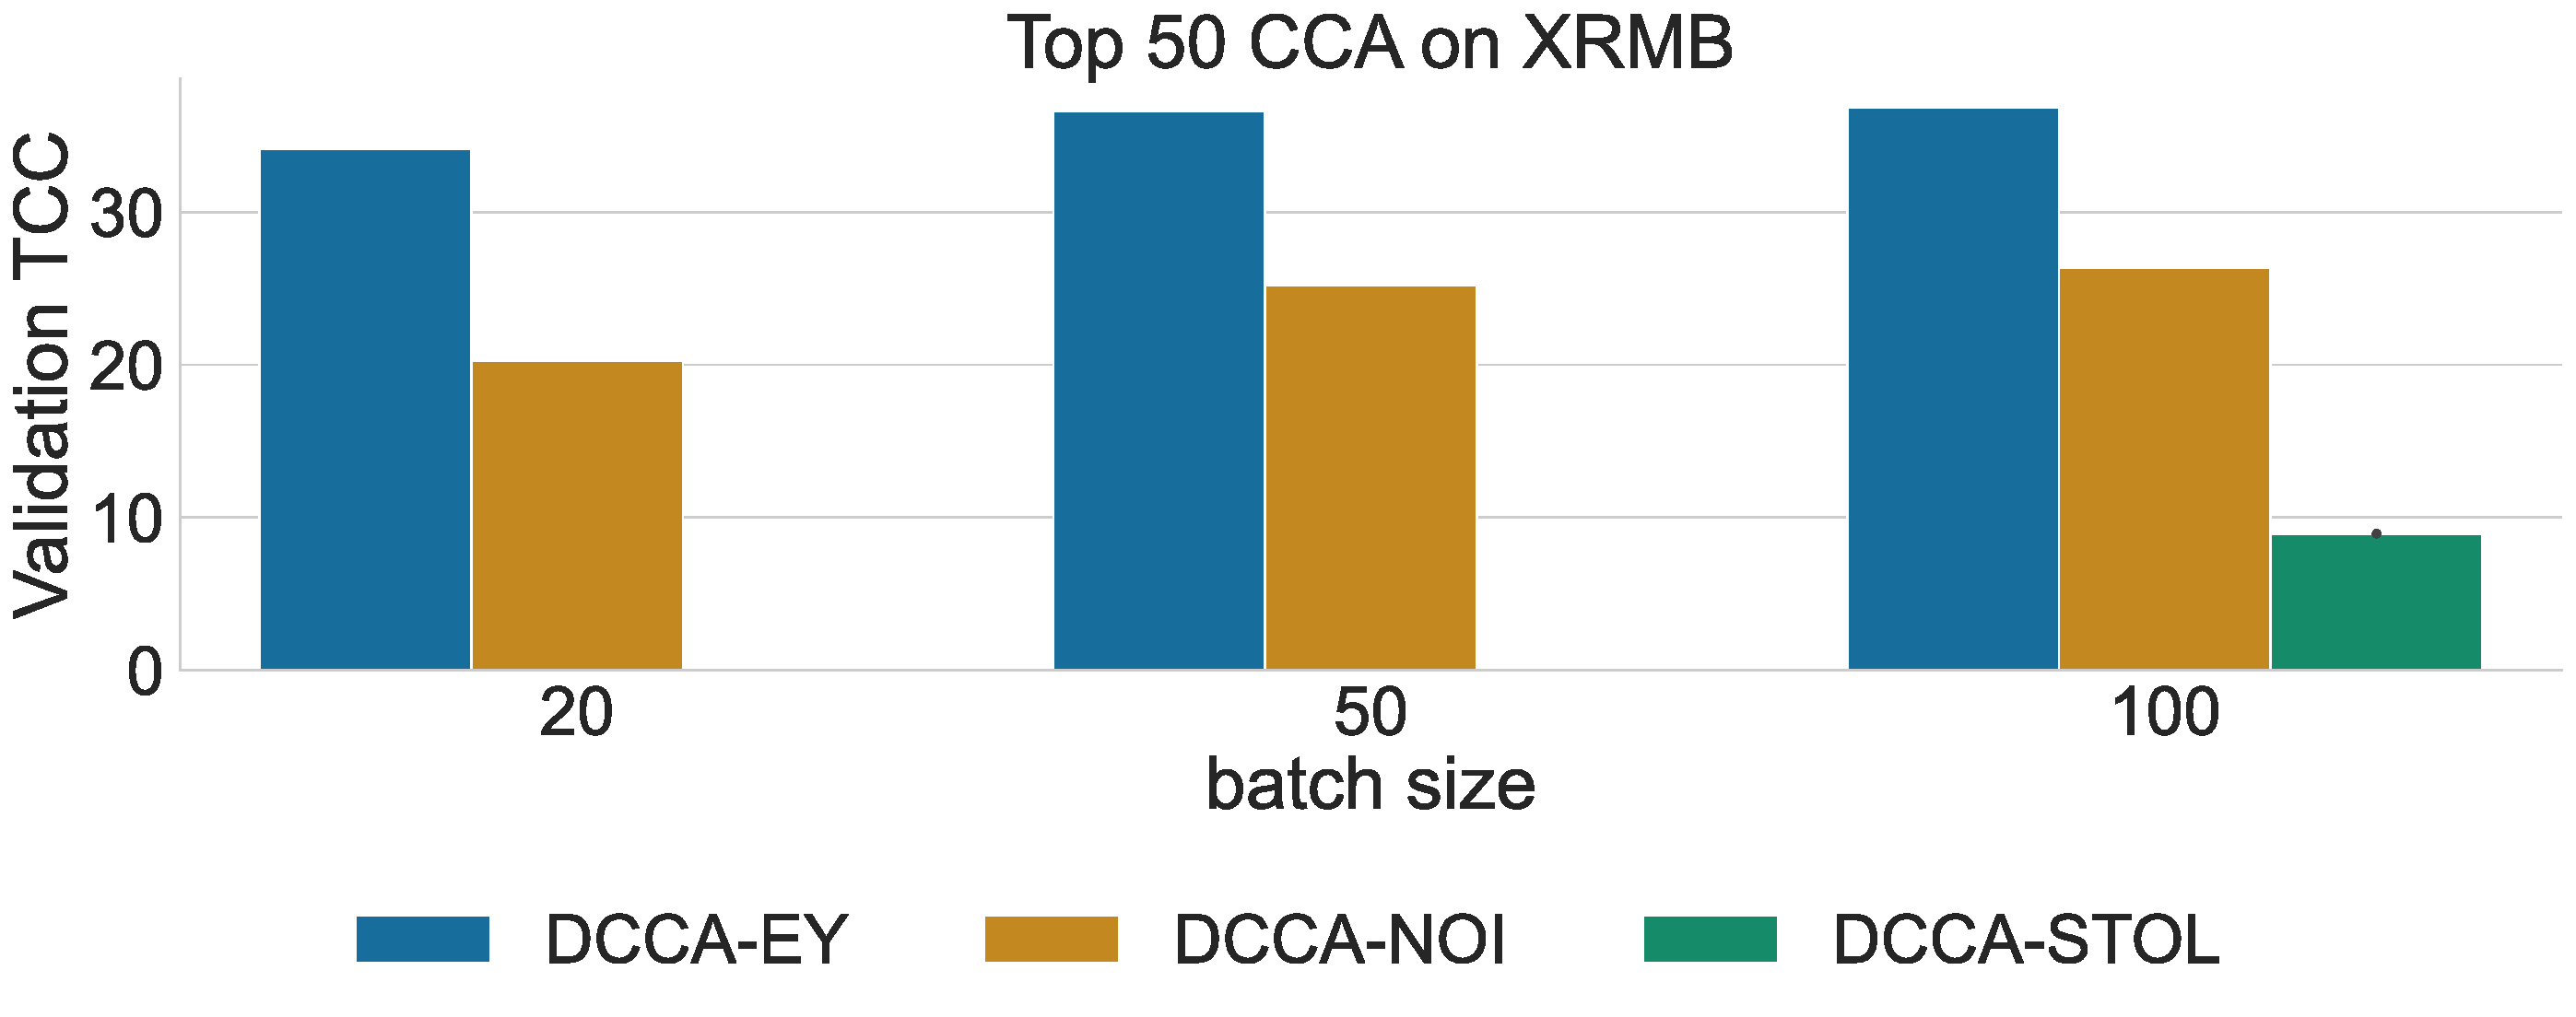
\includegraphics[width=\textwidth]{figures/DCCA/XRMB_models_different_batch_sizes}
        \caption{}
        \label{fig:corr_xrmb}
    \end{subfigure}
    \hfill
    \begin{subfigure}[b]{0.49\textwidth}
        \centering
        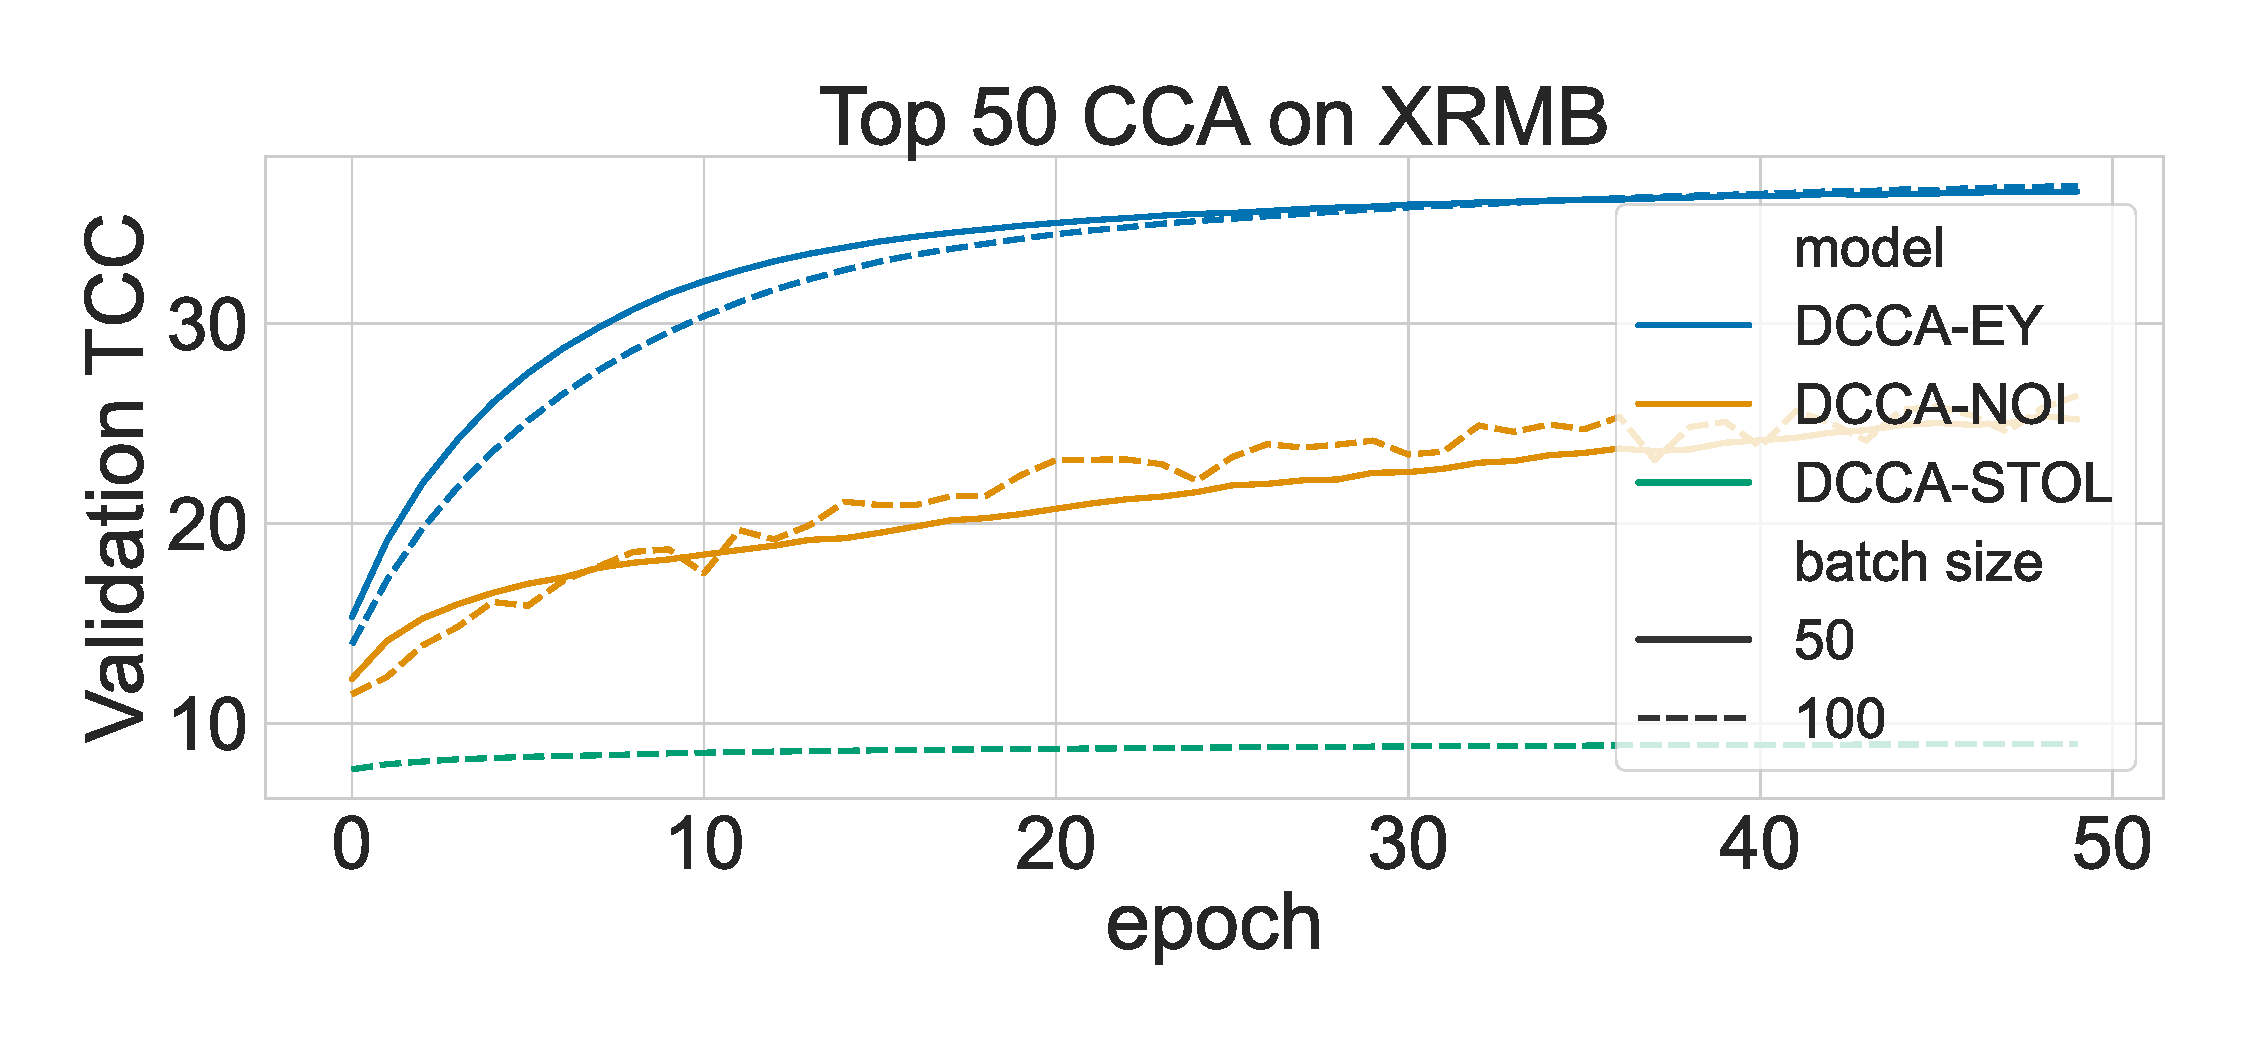
\includegraphics[width=\textwidth]{figures/DCCA/XRMB_allbatchsizes_pcc}
        \caption{}
        \label{fig:lr_xrmb}
    \end{subfigure}
    \caption{Deep CCA on XRMB using the Validation TCC metric: (a) after training each model for 50 epochs with varying batch sizes; (b) learning progress over 50 epochs.}
    \label{fig: xrmb}
\end{figure}

\subsection{Deep Multiview CCA: Robustness Across Different Batch Sizes}
Third, we compare DCCA-EY to the existing DMCCA and DGCCA methods on the mfeat dataset; this contains 2,000 handwritten numeral patterns across six distinct feature sets, including Fourier coefficients, profile correlations, Karhunen-Love coefficients, pixel averages in \(2 \times 3\) windows, Zernike moments, and morphological features. We again learn $K=50$ dimensional representations, but now train for 100 epochs.
We use a multiview extension of the TCC metric, which averages correlation across views; we call this Total Multiview Correlation Captured (TMCC), defined as \(
\text{TMCC} = \sum_{k=1}^{K} \frac{1}{I(I-1)} \sum_{i,j \leq I, i\neq j} \text{corr}(Z_k^{(i)}, Z_k^{(j)}),
\) %where \(Z_k^{(i)}\) is the \(k\)-th dimension of the \(i\)-th view's representation,
using the notation of \cref{sec:background-unified}.

\textbf{Parameters:} For each method, we searched over a hyperparameter grid using \citet{wandb}.

\begin{table}[h!]
    \centering
    \begin{tabular}{|l|l|}
        \hline Parameter      & Values                       \\
        \hline minibatch size & 5,10,20,50,100,200           \\
        \hline components     & 50                           \\
        \hline epochs         & 100                          \\
        \hline lr             & 0.01, 0.001, 0.0001, 0.00001 \\
        \hline
    \end{tabular}
\end{table}

\textbf{Observations:}
Figure~\ref{fig:dmcca_corr} shows that DCCA-EY consistently outperforms both DGCCA and DMCCA across various mini-batch sizes in capturing validation TMCC.
Just like DCCA-NOI, DMCCA breaks down when the batch size is smaller than $K$. This is due to singular empirical covariances; DGCCA does not break down, but does significantly underperform with smaller batch sizes.
This limits their practical applicability to large-scale data.
Figure~\ref{fig:dmcca_lr} shows learning curves for batch sizes 50 and 100.
DMCCA and DGCCA both quickly learn significant correlations but then plateau out; our method consistently improves, and significantly outperforms them by the end of training.

\begin{figure}
    \centering
    \begin{subfigure}[b]{0.49\textwidth}
        \centering
        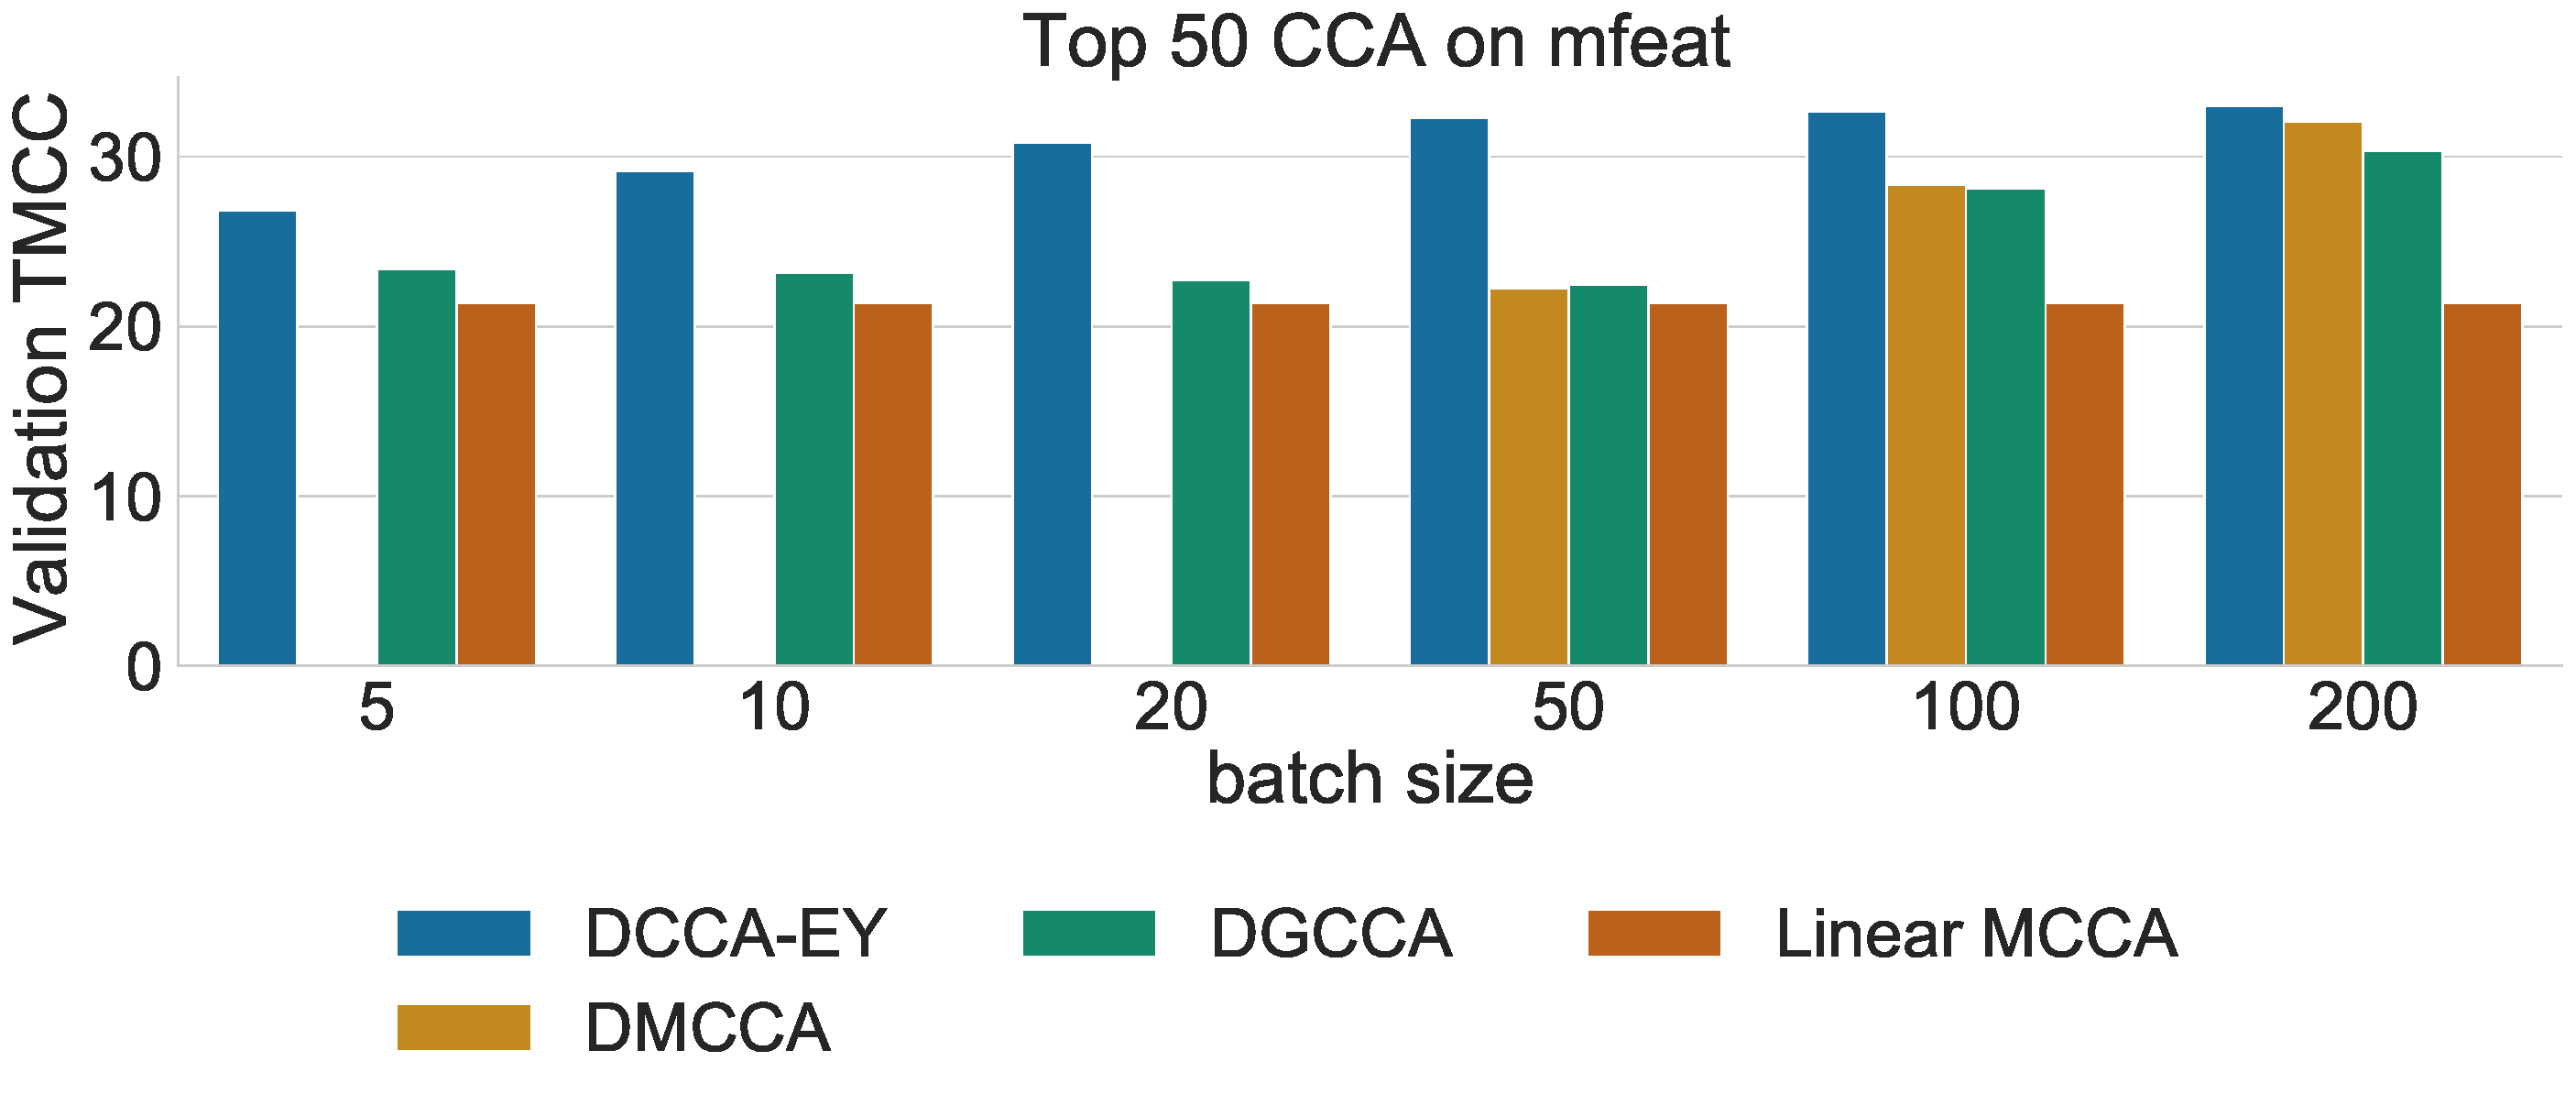
\includegraphics[width=\textwidth]{figures/DMCCA/mfeat_models_different_batch_sizes}
        \caption{}\label{fig:dmcca_corr}
    \end{subfigure}
    \hfill
    \begin{subfigure}[b]{0.49\textwidth}
        \centering
        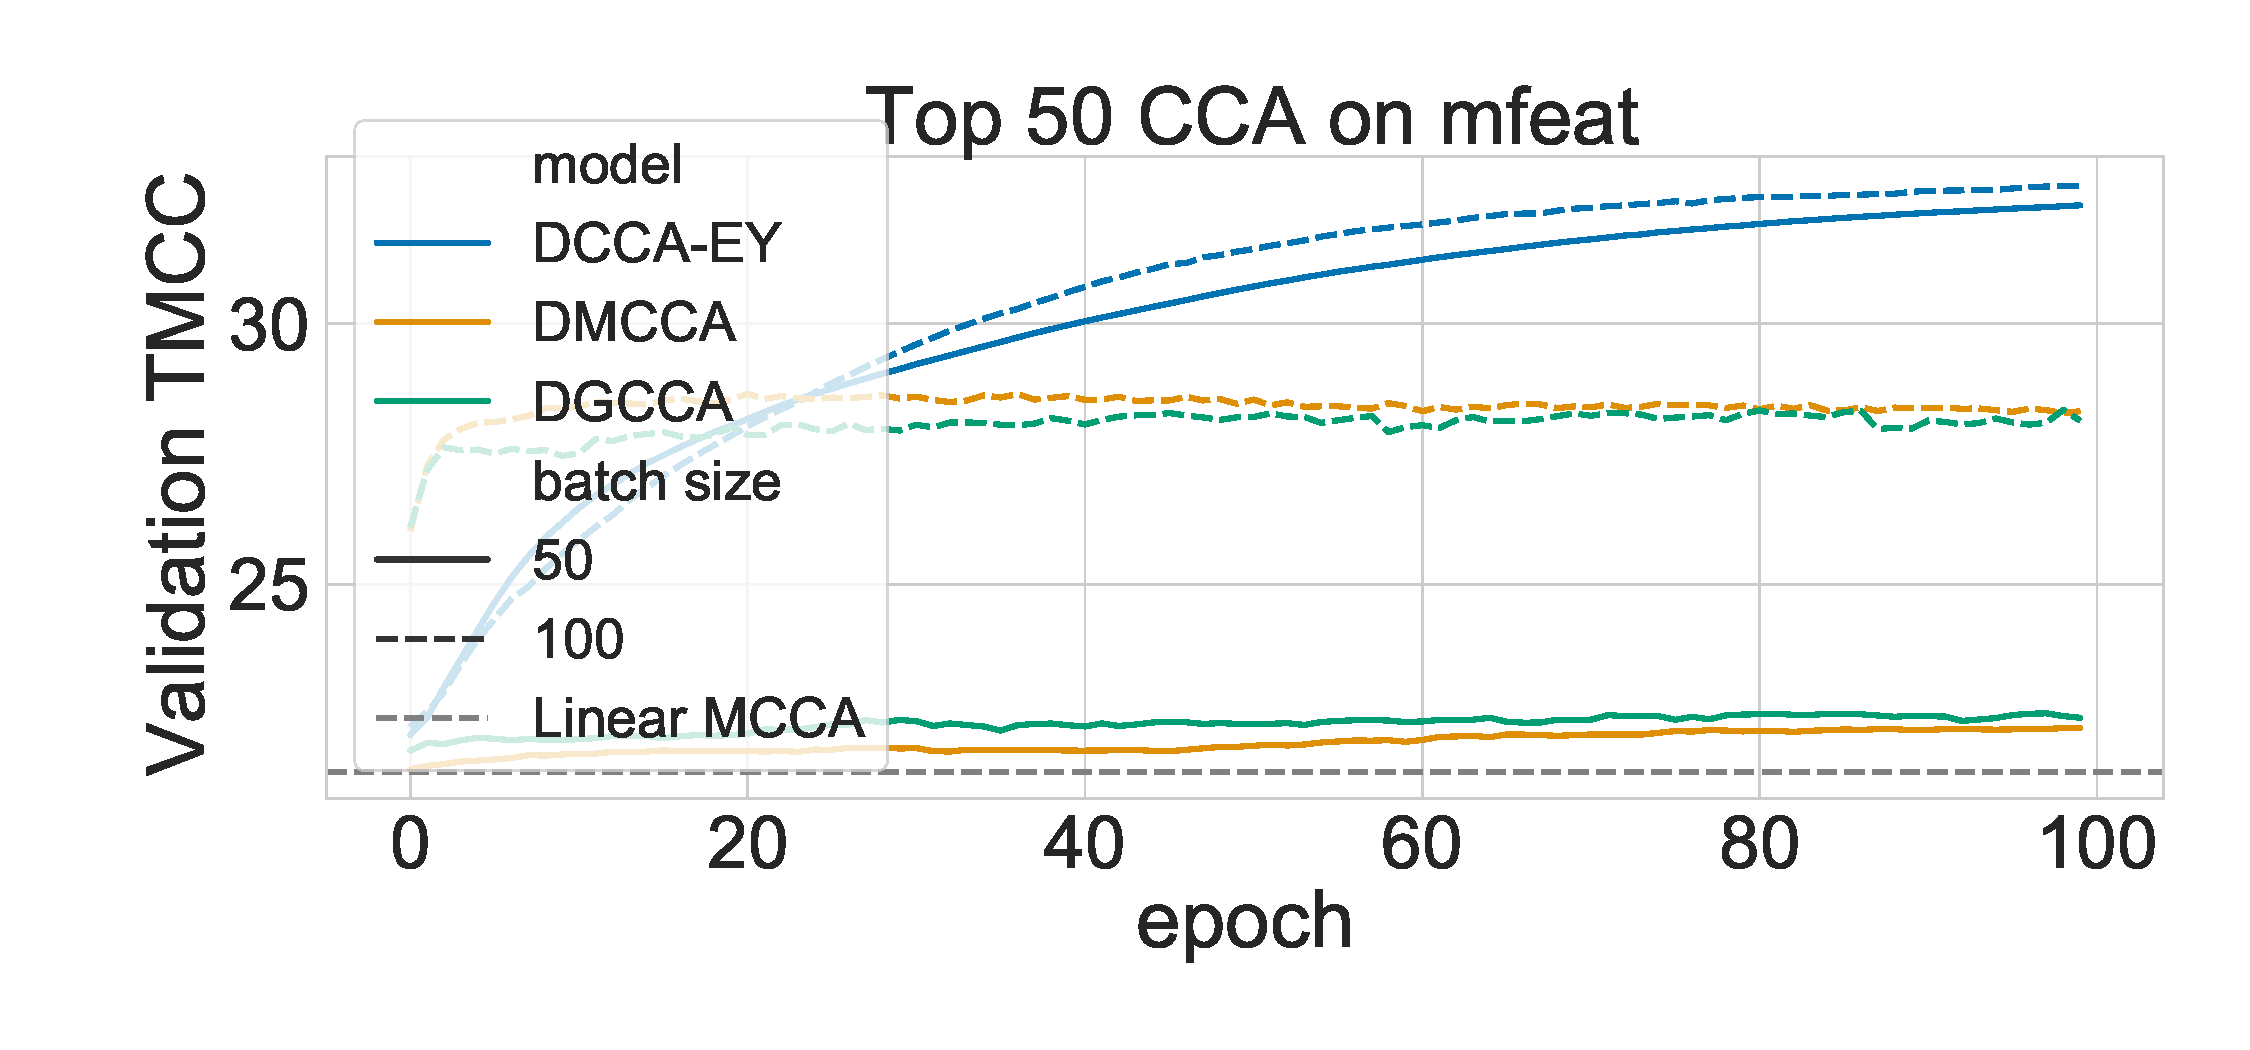
\includegraphics[width=\textwidth]{figures/DMCCA/mfeat_allbatchsizes_pcc}
        \caption{}\label{fig:dmcca_lr}
    \end{subfigure}
    \caption{Deep Multi-view CCA on mfeat using the Validation TMCC metric: (a) after training each model for 100 epochs with varying batch sizes; (b) learning progress over 100 epochs.}
    \label{fig:dmcca}
\end{figure}

\subsection{Self-Supervised Learning with SSL-EY}
Finally, we benchmark our self-supervised learning algorithm, SSL-EY, with Barlow Twins and VICReg on CIFAR-10 and CIFAR-100. Each dataset contains 60,000 labelled images, but these are over 10 classes for CIFAR-10 and 100 classes for CIFAR-100.

We follow a standard experimental design \citep{tong2023emp}. Indeed, we use the sololearn library \citep{da2022solo}, which offers optimized setups particularly tailored for VICReg and Barlow Twins. All methods utilize a ResNet-18 encoder coupled with a bi-layer projector network. Training spans 1,000 epochs with batches of 256 images. For SSL-EY, we use the hyperparameters optimized for Barlow Twins, aiming not to outperform but to showcase the robustness of our method.
We predict labels via a linear probe on the learnt representations and evaluate performance with Top-1 and Top-5 accuracies on the validation set. For more details, refer to the supplementary material \ref{supp:experimental details}.

\textbf{Observations:} Table \ref{tab:selfsup} shows that SSL-EY is competitive with Barlow Twins and VICReg. This is remarkable because we used out-of-the-box hyperparameters for SSL-EY but used hyperparameters for Barlow Twins and VICReg that had been heavily optimized in previous studies.

\begin{table}
    \centering
    \begin{tabular}{lcccc}
        \hline
        Method          & CIFAR-10 Top-1 & CIFAR-10 Top-5 & CIFAR-100 Top-1 & CIFAR-100 Top-5 \\
        \hline
        Barlow Twins    & \textbf{92.1}  & 99.73          & \textbf{71.38}  & \textbf{92.32}  \\
        VICReg          & 91.68          & 99.66          & 68.56           & 90.76           \\
        \textbf{SSL-EY} & 91.43          & \textbf{99.75} & 67.52           & 90.17           \\
        \hline
    \end{tabular}
    \caption{Performance comparison of SSL methods on CIFAR-10 and CIFAR-100.}
    \label{tab:selfsup}
\end{table}


\section{Further Experiments with CIFAR-10 and CIFAR-100}\label{sec:experiments}

\textbf{Model Convergence:} The Learning curves in Figure~\ref{fig:ssl learning curve cifar100 top5} indicate that the performance variation at 1,000 epochs in table \ref{tab:selfsup} mainly results from optimization noise and speed of convergence is similar.

\textbf{Smaller Projector or None at All:}
One key motivation for projectors is to prevent excessive collapse of meaningful information. Because SSL-EY learns does not suffer from collapse, we had a prior that it may be more robust to projector size, and perhaps even to removing the projector altogether.
For this reason, in another set of experiments, we explored varying the projector's output dimensions from 2048 to 64 and removing the projector completely while holding the encoder output size constant. Figure~\ref{fig: ssl projector dimensions 100} demonstrates that SSL-EY maintains good performance even with a smaller projector, making the representations more efficient than Barlow Twins and VICReg (they contain the same amount of useful information for the classification task in much fewer dimensions). While Figure~\ref{fig: ssl projector dimensions 100} shows the strong performance of Barlow Twins and VICReg at larger projector sizes for this task, we would argue that our objective is more robust to this design choice, potentially offering a more reliable choice for practitioners employing SSL to unfamiliar datasets. At the bottom of Table \ref{tab:selfsup}, we further highlight the efficiency of SSL-EY by showing that our model performs similarly when we have no projector (just using the a 2048 dimensional representation), suggesting that SSL-EY is less reliant on this architecture\footnote{We note that W-MSE, a close relative of our work, also didn't use a projector despite its use being seemingly ubiquitous}. In contrast, we show in appendix \ref{sec:noproj} that Barlow Twins and VICReg's performance drops substantially without the use of a projector.

\textbf{$\LEY$ is an informative metric:} Figure~\ref{fig:ssl learning curve cifar100 vs corr} offers two key insights. First, it shows that the EY loss, which provides an unbiased estimate of the canonical correlations of the embeddings, is closely related to classification accuracy. This suggests that maximizing canonical correlation is a promising pretext task for self-supervised learning. Second, the figure reveals that even a reduced-dimensionality projector output (64 dimensions) has not reached its full capacity by 1,000 epochs. Specifically, the sum of squared canonical correlations reaches 46, out of a maximum possible value of 64. This indicates that there is still room for further optimization, implying that SSL-EY's representations have not yet saturated their capacity for capturing meaningful information. Lastly, the evolution of the correlation, as measured by $\LEY$, offers a novel way of monitoring model training even without the need for a separate validation task like classification, and could potentially eliminate the requirement for a validation set altogether. This is a particularly interesting direction given recent work on the stepwise eigenvalue behavior of the representations in SSL models \cite{simon2023stepwise}.

\begin{table}[H]
    \centering
    \begin{tabular}{lcccc}
        \hline
        Method          & CIFAR-10 Top-1 & CIFAR-10 Top-5 & CIFAR-100 Top-1 & CIFAR-100 Top-5 \\
        \hline
        Barlow Twins    & \textbf{92.1}  & 99.73          & \textbf{71.38}  & \textbf{92.32}  \\
        VICReg          & 91.68          & 99.66          & 68.56           & 90.76           \\
        \textbf{SSL-EY} & 91.43          & \textbf{99.75} & 67.52           & 90.17           \\
        \hline
        SSL-EY No Proj. & 90.98          & 99.69          & 65.21           & 88.09           \\
        \hline
    \end{tabular}
    \caption{Performance comparison of SSL methods on CIFAR-10 and CIFAR-100.}
    \label{tab:selfsup}
\end{table}

\begin{figure}[H]
    \centering
% 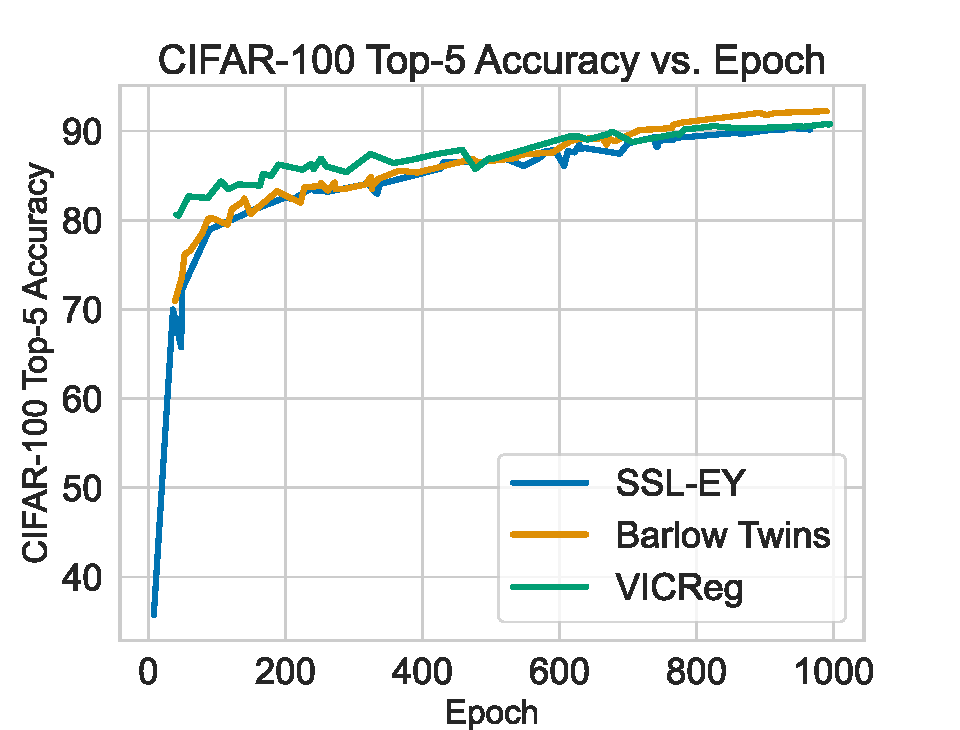
\includegraphics[width=\textwidth]{figures/SSL/cifar100_top5_learning_curve.svg}
    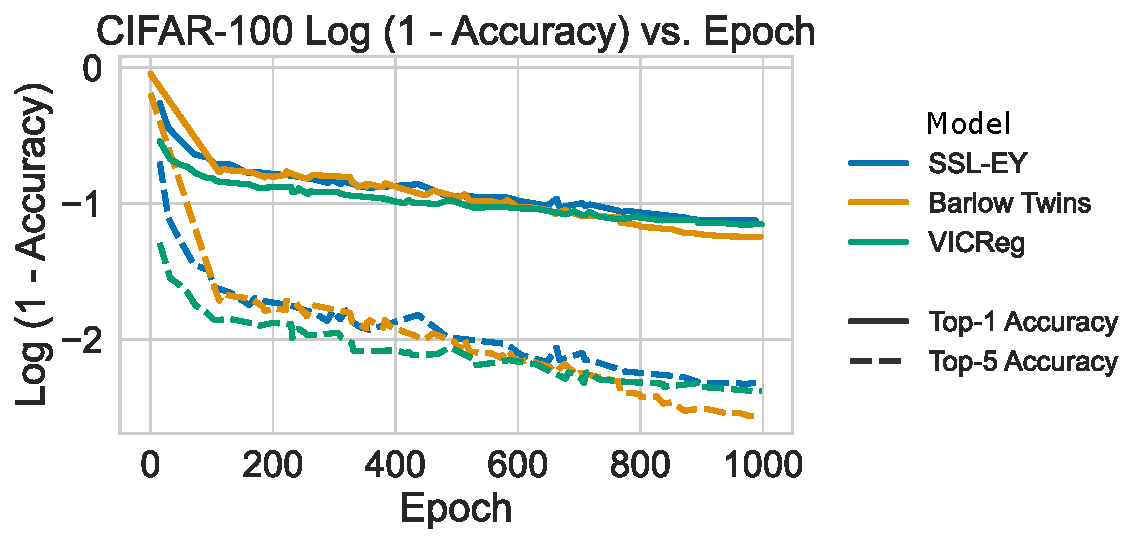
\includegraphics[width=0.57\textwidth]{figures/SSL/cifar100_learning_curve_log_error}
    \caption{Learning curves for SSL-EY, Barlow Twins, and VICReg on CIFAR-100, showing performance across 1,000 epochs.}
    \label{fig:ssl learning curve cifar100 top5}
\end{figure}

\begin{figure}[H]
    \begin{subfigure}[b]{0.47\textwidth}
        \centering
        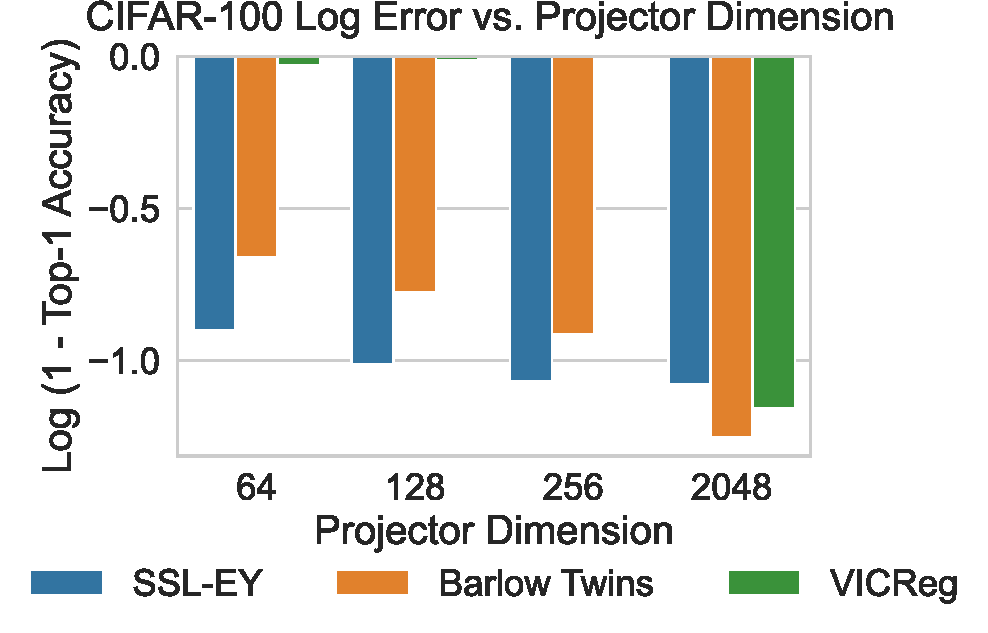
\includegraphics[width=\textwidth]{figures/SSL/cifar100_proj_dim_log_error}
        \caption{}
        \label{fig: ssl projector dimensions 100}
    \end{subfigure}
    \begin{subfigure}[b]{0.47\textwidth}
        \centering
        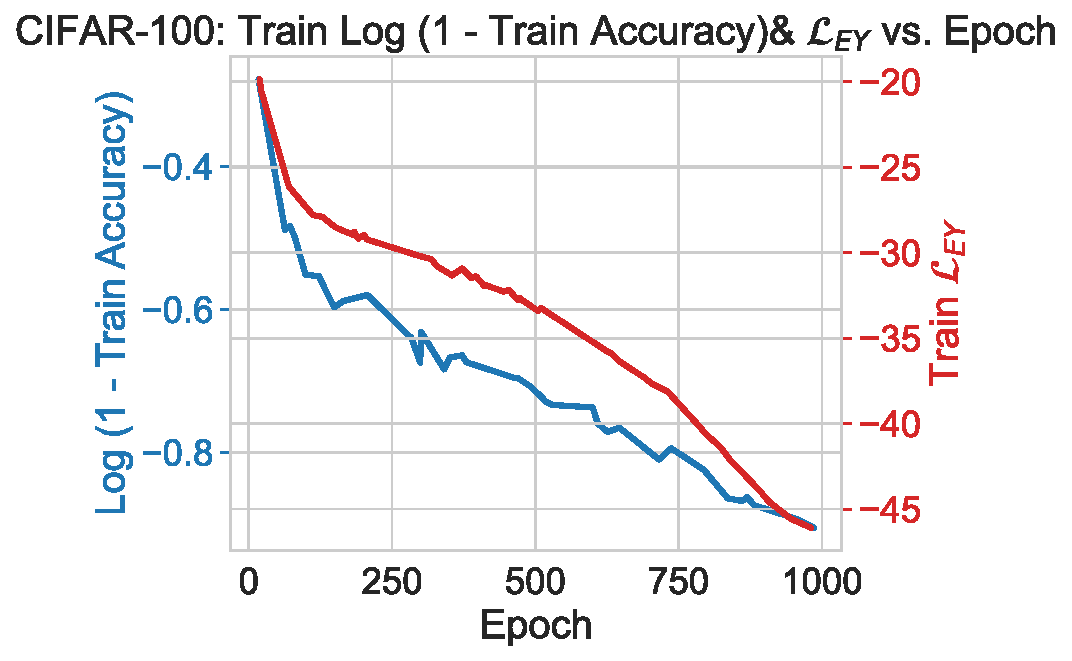
\includegraphics[width=\textwidth]{figures/SSL/cifar100_corr_vs_acc_log_error}
        \caption{}
        \label{fig:ssl learning curve cifar100 vs corr}
    \end{subfigure}
    \caption{(a) Performance of SSL-EY with reduced projector size compared to Barlow Twins and VICReg. (b) SSL-EY's learned embeddings indicate untapped representation capacity.}
    \label{fig: ssl projector cifar 100}
\end{figure}